\documentclass[12pt,a4paper]{article}
\usepackage[utf8]{inputenc}
\usepackage[T1]{fontenc}
\usepackage{lmodern}
\usepackage[brazil]{babel}
\usepackage{geometry}
\usepackage{booktabs}
\usepackage{xcolor}
\usepackage{listings}
\usepackage{graphicx}
\graphicspath{{UVM/DOT/doc_verif/}{./}}
\usepackage{enumitem}
\usepackage{float}
\usepackage{array}
\usepackage{tabularx}
\usepackage{longtable}
\usepackage{amsmath}
\usepackage[hidelinks]{hyperref}

\geometry{landscape, margin=2.2cm}
\setlength{\parindent}{0pt}
\setlength{\parskip}{0.45em}
\renewcommand{\arraystretch}{1.15}



\title{Requisitos de Verificação -- Bloco DotProduct}
\author{Matheus Grossi}
\date{2026}
\hypersetup{pdftitle={Requisitos de Verificação -- DotProduct},pdfauthor={Matheus Grossi}}
\begin{document}
\maketitle
\vspace{1.5cm}
\section{Identificação do Bloco}
\begin{itemize}[label=\textbullet]
\item \textbf{1.1. Nome do bloco:} DotProduct (DOT), unidade de produto escalar de 32 elementos signed de 8 bits, com acumulador de 21 bits.
\item \textbf{1.2. Versão:} não informada no plano de verificação do DOT.
\item \textbf{1.3. Autor do bloco:} não informado no plano de verificação do DOT.
\item \textbf{1.4. Responsável pela verificação:} Matheus Grossi.
\item \textbf{1.5. Escopo da verificação:} correção matemática, interpretação signed, indexação, reset, validade, ordenação, perda/duplicação, estados X/Z e latência por transação.
\end{itemize}

\section{Objetivo da Verificação}
Verificar que o DotProduct calcule corretamente a soma dos produtos entre os elementos de entrada e os pesos:
\[
expected=\sum_{i=0}^{31} input\_vec[i]\times weight[i].
\]
A configuração considerada utiliza \texttt{DATA\_WIDTH=8}, \texttt{N\_INPUTS=32} e \texttt{ACC\_WIDTH=21}. Cada vetor possui 256 bits. O clock tem período de 10 ns; são consideradas seis posições de ocupação do pipeline e cinco ciclos entre a captura da entrada e a saída válida.

Além do resultado aritmético, devem ser verificados o ciclo de saída, a validade e a ordem de cada operação. O reset atua sobre o pipeline de validade; não se exige que ele zere o datapath. A primeira aparição do dado e a de \texttt{valid\_out} são medidas separadamente nos testes dirigidos de latência.

\section{Estratégia de Verificação}
A estratégia combina testes dirigidos, varreduras de subespaços e amostragem aleatória com sementes registradas. As rotinas são:
\begin{enumerate}
\item Reset inicial e reset durante atividade;
\item Varreduras com 1, 4, 8 e 12 elementos ativos, em quatro rodadas por teste;
\item Padrões contendo X, Z e alternância X/Z;
\item Entradas ou pesos zero, elemento unitário e indexação das 32 posições;
\item Extremos signed, sinais alternados e cancelamento perfeito;
\item Operação contínua, gaps e padrão conhecido de validade;
\item Impulso único, latência após reset e ocupações de um a seis pacotes com padrões zero, um e alternados.
\end{enumerate}
O scoreboard utiliza uma referência independente e associa cada transação ao ciclo esperado, verificando dado e validade separadamente. Assertions procedurais e cobertura funcional complementam as comparações. IDs, rodadas e sementes são registrados para permitir a investigação de falhas. T02--T06 totalizam 281.600 transações principais; cada uma também é uma verificação temporal.

\section{Casos de Teste Executados / Planejados}
A matriz apresenta os estímulos e os resultados exigidos. Todos os casos devem respeitar a validade e a latência especificadas; a análise da execução aparece na seção de análise dos resultados.
\small
\begin{longtable}{|p{1.1cm}|p{4.5cm}|p{7cm}|p{10cm}|}
\hline\textbf{Caso} & \textbf{Condição} & \textbf{Estímulo} & \textbf{Resultado esperado}\\\hline
\endfirsthead
\hline\textbf{Caso} & \textbf{Condição} & \textbf{Estímulo} & \textbf{Resultado esperado}\\\hline
\endhead
T00 & Reset inicial & Reset ativo e primeira operação após liberação & Nenhuma saída válida durante reset; primeira operação com latência nominal. \\\hline
T01 & Reset durante atividade & Operações em trânsito, reset e nova operação & Invalidar as operações anteriores; preservar a latência após reset. \\\hline
T02 & Um elemento de 8 bits & 4 rodadas de 256 valores; pesos 0--31 & Produto escalar signed correto em cada ciclo esperado. \\\hline
T03 & Quatro elementos de 4 bits & 4 rodadas de 256 casos; pesos 0--15 & Soma dos quatro produtos correta, com validade e latência nominais. \\\hline
T04 & Oito elementos de 1 bit & 4 rodadas das 256 combinações; pesos 0--3 & Soma correta para todas as combinações binárias aplicadas. \\\hline
T05 & Quatro elementos de 8 bits & 4 rodadas de 4.096 amostras; pesos 0--31 & Resultado signed correto, sem perda ou duplicação. \\\hline
T06 & Doze elementos de 4 bits & 4 rodadas de 65.536 amostras; pesos 0--31 & Resultado e ciclo de saída corretos nas 262.144 transações. \\\hline
T07 & Entrada X & Um elemento X; peso conhecido aleatório & Resultado desconhecido no ciclo nominal. \\\hline
T08 & Entrada Z & Um elemento Z; peso conhecido aleatório & Propagação de desconhecido pela operação aritmética. \\\hline
T09 & Z alternado & Quatro padrões alternando bits conhecidos e Z & Estado desconhecido associado à transação no ciclo esperado. \\\hline
T10 & Z com pesos X/Z & Entrada Z e dois padrões de pesos X/Z & Resultado desconhecido com validade e latência corretas. \\\hline
T11 & Z alternado com pesos X/Z & Dois padrões mistos de entrada e pesos & Propagação de desconhecido no ciclo esperado. \\\hline
T12 & Entradas zero & 32 vetores de pesos aleatórios & Saída zero no ciclo válido nominal. \\\hline
T13 & Pesos zero & 32 vetores de entrada aleatórios & Saída zero no ciclo válido nominal. \\\hline
T14 & Elemento unitário & 256 valores signed com peso 1 & Saída igual ao elemento aplicado. \\\hline
T15 & Walking element & Valor 37 e peso 1 em cada uma das 32 posições & Saída 37, independentemente da posição. \\\hline
T16 & Extremos signed & Quatro combinações entre 127 e -128 & Multiplicação e extensão de sinal corretas. \\\hline
T17 & Máximo positivo & Todos os pares de elementos iguais a 127 & Saída 516.128 sem overflow indevido. \\\hline
T18 & Mínimo negativo nos operandos & Todos os pares de elementos iguais a -128 & Saída 524.288 sem overflow indevido. \\\hline
T19 & Sinais alternados & Dois padrões de sinais nos operandos & Soma signed correta, inclusive cancelamentos. \\\hline
T20 & Cancelamento perfeito & Quatro produtos 10, -10, 10, -10 & Saída exatamente zero. \\\hline
T21 & Back-to-back & 256 operações válidas consecutivas & Um resultado por ciclo, na ordem, sem perda ou duplicação. \\\hline
T22 & Gaps em valid & 256 ciclos com gaps pseudoaleatórios & Somente entradas válidas geram saídas válidas, com deslocamento nominal. \\\hline
T23 & Impulso único & Uma operação reconhecível: 7 vezes 3 & Saída 21; primeira aparição de dado e validade após cinco ciclos. \\\hline
T24 & Padrão conhecido de valid & Padrão 1 0 1 1 0 0 1 0 1 & Repetir o padrão na saída, deslocado pela latência nominal. \\\hline
T25 & Latência após reset & Operação reconhecível após reset & Latências de dado e validade iguais às medidas em T23. \\\hline
T26 & Pacotes zero & Ocupações 1--6, seis pacotes válidos por subcaso & 36 resultados zero, todos no ciclo esperado. \\\hline
T27 & Pacotes em um & Ocupações 1--6; slots restantes zerados & 36 resultados signed corretos e temporalmente alinhados. \\\hline
T28 & Pacotes alternados & Padrão 01010101; ocupações 1--6 & 36 resultados corretos, com slots restantes zerados e latência nominal. \\\hline
\end{longtable}
\normalsize

\section{Casos de Fronteira}
\begin{table}[H]\centering\small
\begin{tabularx}{\textwidth}{p{4cm}Xp{5cm}}\toprule
\textbf{Condição} & \textbf{Estímulo} & \textbf{Resultado esperado}\\\midrule
Entradas ou pesos zero & Um vetor zerado e o outro com valores conhecidos aleatórios & Zero no ciclo nominal.\\
Elemento unitário e indexação & Peso 1; valores signed e walking element de valor 37 nas 32 posições & Próprio elemento; 37 em cada posição.\\
Extremos signed & $127\times127$, $127\times(-128)$, $(-128)\times127$, $(-128)\times(-128)$ & 16.129; $-16.256$; $-16.256$; 16.384.\\
Todos os elementos extremos & 32 pares $(127,127)$ ou $(-128,-128)$ & 516.128 ou 524.288, sem overflow indevido.\\
Cancelamento & Sinais alternados; quatro produtos $10,-10,10,-10$ & Resultado da soma signed; zero no cancelamento perfeito.\\
Reset durante atividade & Quatro operações em trânsito, reset e uma nova operação & Quatro descartes; operação posterior com latência nominal.\\
Estados X/Z & Entradas desconhecidas ou alta impedância e pesos conhecidos/mistos & Propagação de desconhecidos no ciclo nominal; pendente de execução em quatro estados.\\\bottomrule
\end{tabularx}
\caption{Fronteiras aritméticas, estruturais e temporais exercitadas ou previstas.}
\end{table}


\section{Resultados}
\subsection{Comportamentos esperados}
Cada entrada válida deve produzir o produto escalar signed correto após cinco ciclos, com \texttt{valid\_out} ativo no ciclo correspondente. Operações consecutivas devem manter a ordem e o throughput, sem perda ou duplicação; gaps devem ser reproduzidos no pipeline de validade.

Entradas ou pesos conhecidos inteiramente zerados devem produzir zero. A indexação e os extremos devem preservar a interpretação signed e a largura do acumulador. Nos testes X/Z, o resultado desconhecido deve corresponder à transação e ao ciclo previstos. Após reset, as operações invalidadas não devem reaparecer como válidas, e novas operações devem manter a característica temporal.

\subsection{Critério de aprovação}
O bloco será considerado aprovado quando:
\begin{itemize}
\item todos os casos obrigatórios e as quatro rodadas das varreduras forem executados;
\item as 281.600 transações principais e os casos dirigidos tiverem as contagens previstas;
\item os resultados matemáticos, signed, extremos e cancelamentos forem corretos;
\item as 32 posições e todas as classes obrigatórias de cobertura forem exercitadas;
\item os estados X/Z apresentarem o comportamento esperado;
\item dado e validade respeitarem a latência exigida e a ordem das transações;
\item reset e gaps não introduzirem perda, duplicação ou deslocamento temporal indevido;
\item as assertions e comparações não apresentarem falhas.
\end{itemize}
Um valor matematicamente correto não elimina uma falha temporal. Testes obrigatórios pulados impedem a aprovação completa.

\section{Análise dos Resultados}
\subsection{Interpretação dos casos de sucesso/falha}
\textbf{Sucesso:} valor, validade, ordem e latência atendem ao comportamento exigido para o caso.\par
\textbf{Falha:} ocorre divergência matemática, temporal, de validade, ordem ou estado desconhecido.\par
\textbf{SKIP:} caso obrigatório não executado; não representa aprovação.

A execução em Verilator 5.050 registrou os resultados abaixo. A coluna ``Checadas'' contabiliza comparações aprovadas de dados; T23 apresenta comparação matemática correta, mas falha na caracterização temporal.
\small
\begin{longtable}{p{1cm}p{9cm}rrrp{2cm}}
\toprule \textbf{ID} & \textbf{Caso} & \textbf{Aplicadas} & \textbf{Checadas} & \textbf{Descartadas} & \textbf{Resultado}\\\midrule
\endfirsthead
\toprule \textbf{ID} & \textbf{Caso} & \textbf{Aplicadas} & \textbf{Checadas} & \textbf{Descartadas} & \textbf{Resultado}\\\midrule
\endhead
T00 & Reset inicial & 1 & 1 & 0 & PASS \\
T01 & Reset durante atividade & 5 & 1 & 4 & PASS \\
T02 & 1 elemento x 8 bits & 1.024 & 1.024 & 0 & PASS \\
T03 & 4 elementos x 4 bits & 1.024 & 1.024 & 0 & PASS \\
T04 & 8 elementos x 1 bit & 1.024 & 1.024 & 0 & PASS \\
T05 & 4 elementos x 8 bits & 16.384 & 16.384 & 0 & PASS \\
T06 & 12 elementos x 4 bits & 262.144 & 262.144 & 0 & PASS \\
T07 & Entrada em X & 0 & 0 & 0 & SKIP \\
T08 & Entrada em Z & 0 & 0 & 0 & SKIP \\
T09 & Z alternado & 0 & 0 & 0 & SKIP \\
T10 & Z com pesos X/Z & 0 & 0 & 0 & SKIP \\
T11 & Z alternado com pesos X/Z & 0 & 0 & 0 & SKIP \\
T12 & Entradas iguais a zero & 32 & 32 & 0 & PASS \\
T13 & Pesos iguais a zero & 32 & 32 & 0 & PASS \\
T14 & Elemento unitario & 256 & 256 & 0 & PASS \\
T15 & Walking element & 32 & 32 & 0 & PASS \\
T16 & Extremos signed & 4 & 4 & 0 & PASS \\
T17 & Maximo positivo & 1 & 1 & 0 & PASS \\
T18 & Minimo negativo & 1 & 1 & 0 & PASS \\
T19 & Sinais alternados & 2 & 2 & 0 & PASS \\
T20 & Cancelamento perfeito & 1 & 1 & 0 & PASS \\
T21 & Operacoes back-to-back & 256 & 256 & 0 & PASS \\
T22 & Gaps em valid\_in & 169 & 169 & 0 & PASS \\
T23 & Impulso unico & 1 & 1 & 0 & FAIL (1) \\
T24 & Padrao conhecido de valid & 5 & 5 & 0 & PASS \\
T25 & Latencia apos reset & 1 & 1 & 0 & PASS \\
T26 & Latencia - pacotes em zero & 36 & 36 & 0 & PASS \\
T27 & Latencia - pacotes em um & 36 & 36 & 0 & PASS \\
T28 & Latencia - pacotes alternados & 36 & 36 & 0 & PASS \\
\bottomrule
\end{longtable}
\normalsize
\begin{table}[H]\centering
\begin{tabular}{p{12cm}p{8cm}}\toprule
\textbf{Indicador} & \textbf{Resultado registrado}\\\midrule
Transações aplicadas / checadas / descartadas por reset & 282.507 / 282.503 / 4\\
Comparações funcionais PASS / FAIL & 282.503 / 0\\
Latência PASS / FAIL & 282.503 / 1\\
Validade no ciclo esperado PASS / FAIL & 282.503 / 0\\
Ordem T21 & 256 de 256; nenhuma falha\\
Perdas / duplicações & 0 / 0\\
Antecipações / atrasos & 1 / 0\\
Assertions procedurais PASS / FAIL & 283.188 / 0\\
Latência observada nos ciclos válidos: mínima / máxima / média & 5 / 5 / 5 ciclos\\
Primeira aparição em T23 e T25 & Dado: 4 ciclos; validade: 5 ciclos\\
Testes PASS / FAIL / SKIP & 23 / 1 / 5\\
Resultado final & \textbf{INCOMPLETE}\\\bottomrule
\end{tabular}
\caption{Síntese da regressão UVM.}
\end{table}


T23 exige que a primeira aparição do dado e de \texttt{valid\_out} ocorra em cinco ciclos. Foram medidos \textbf{$L_{DATA}=4$ e $L_{VALID}=5$}, resultando em uma falha temporal. Essa ocorrência também está presente no testbench original: os vetores são preparados antes do ciclo de ativação de \texttt{valid\_in}, e o DUT processa os dados a cada clock, inclusive em ciclos inválidos. O dado pode, portanto, aparecer antecipadamente nessa medição.

T25 compara a característica após reset com T23. Como as duas latências permanecem iguais às medidas anteriores, T25 passa. A falha de T23 não foi demonstrada como defeito do simulador e requer análise separada do estímulo e do critério de alinhamento. As estatísticas de dado no ciclo válido são distintas da medição da primeira aparição; por isso podem indicar cinco ciclos enquanto T23 mede quatro para a primeira aparição física.


\subsection{Sumário da cobertura de verificação}
\begin{table}[H]\centering
\begin{tabularx}{\textwidth}{p{7cm}X}\toprule
\textbf{Métrica/grupo} & \textbf{Evidência obtida}\\\midrule
Cobertura de linhas do RTL & \textbf{96,7\% (29 de 30 linhas)}, filtrada para DotProduct.\\
Cobertura de funções e branches & O resumo LCOV informa ausência de dados; não foi atribuída porcentagem.\\
Reset, validade e pipeline & Reset inicial/durante atividade; valid 0/1; operação isolada, contínua e com gaps exercitados.\\
Elementos ativos e signed & Classes 1, 4, 8, 12 e 32; limites signed mínimo/máximo exercitados.\\
Indexação & 32 de 32 posições.\\
Latência e ordem & Latência correta e antecipada observadas; nenhuma atrasada. Ordem correta exercitada, sem reordenação.\\
Estados especiais & X=0, Z=0, XZ=0: não cobertos nessa execução.\\
Grupos obrigatórios de cobertura com falha & Contador 0 sob a política que trata X/Z como SKIP; não implica cobertura completa dos requisitos.\\\bottomrule
\end{tabularx}
\caption{Cobertura de código e cobertura funcional são métricas distintas.}
\end{table}
As evidências quantitativas foram extraídas dos logs do DOT. A taxa de linhas exercitadas não indica aprovação funcional da regressão.

As Figuras \ref{fig:dot-cobertura-geral} e \ref{fig:dot-cobertura-fonte} apresentam as capturas do relatório LCOV do DotProduct. A visão geral registra 29 de 30 linhas exercitadas (96,7\%); o detalhamento mostra os contadores associados às linhas do RTL.

\begin{figure}[H]
    \centering
    \fbox{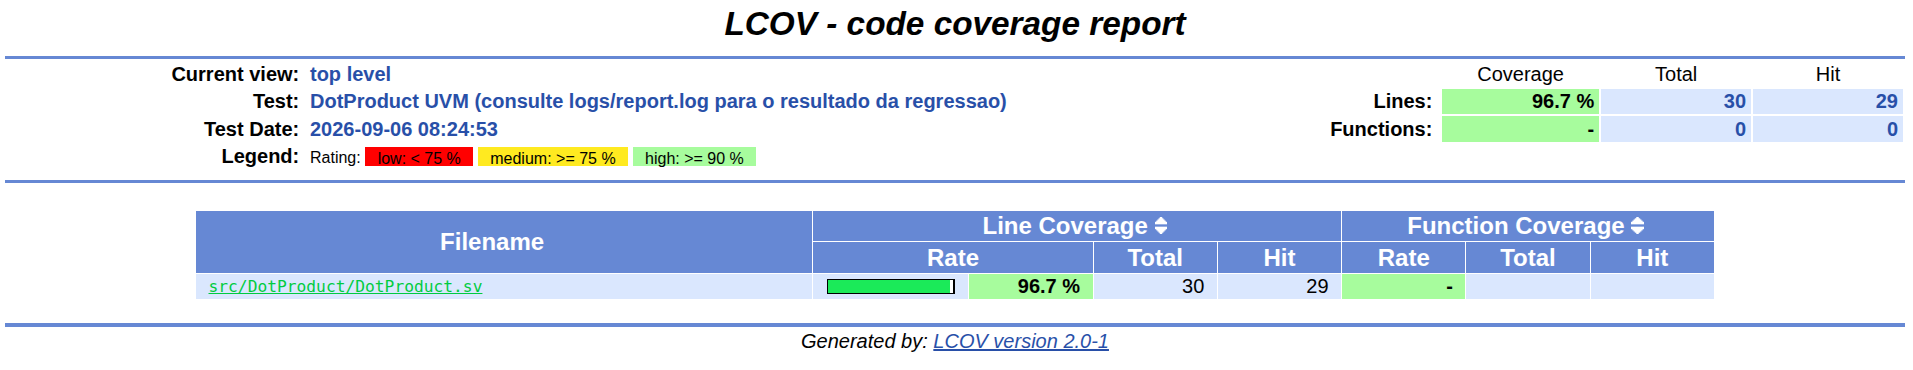
\includegraphics[width=0.94\textwidth]{cap1.png}}
    \caption{Cobertura do DotProduct UVM: visão geral do relatório LCOV (cap1).}
    \label{fig:dot-cobertura-geral}
\end{figure}

\clearpage
\begin{figure}[H]
    \centering
    \fbox{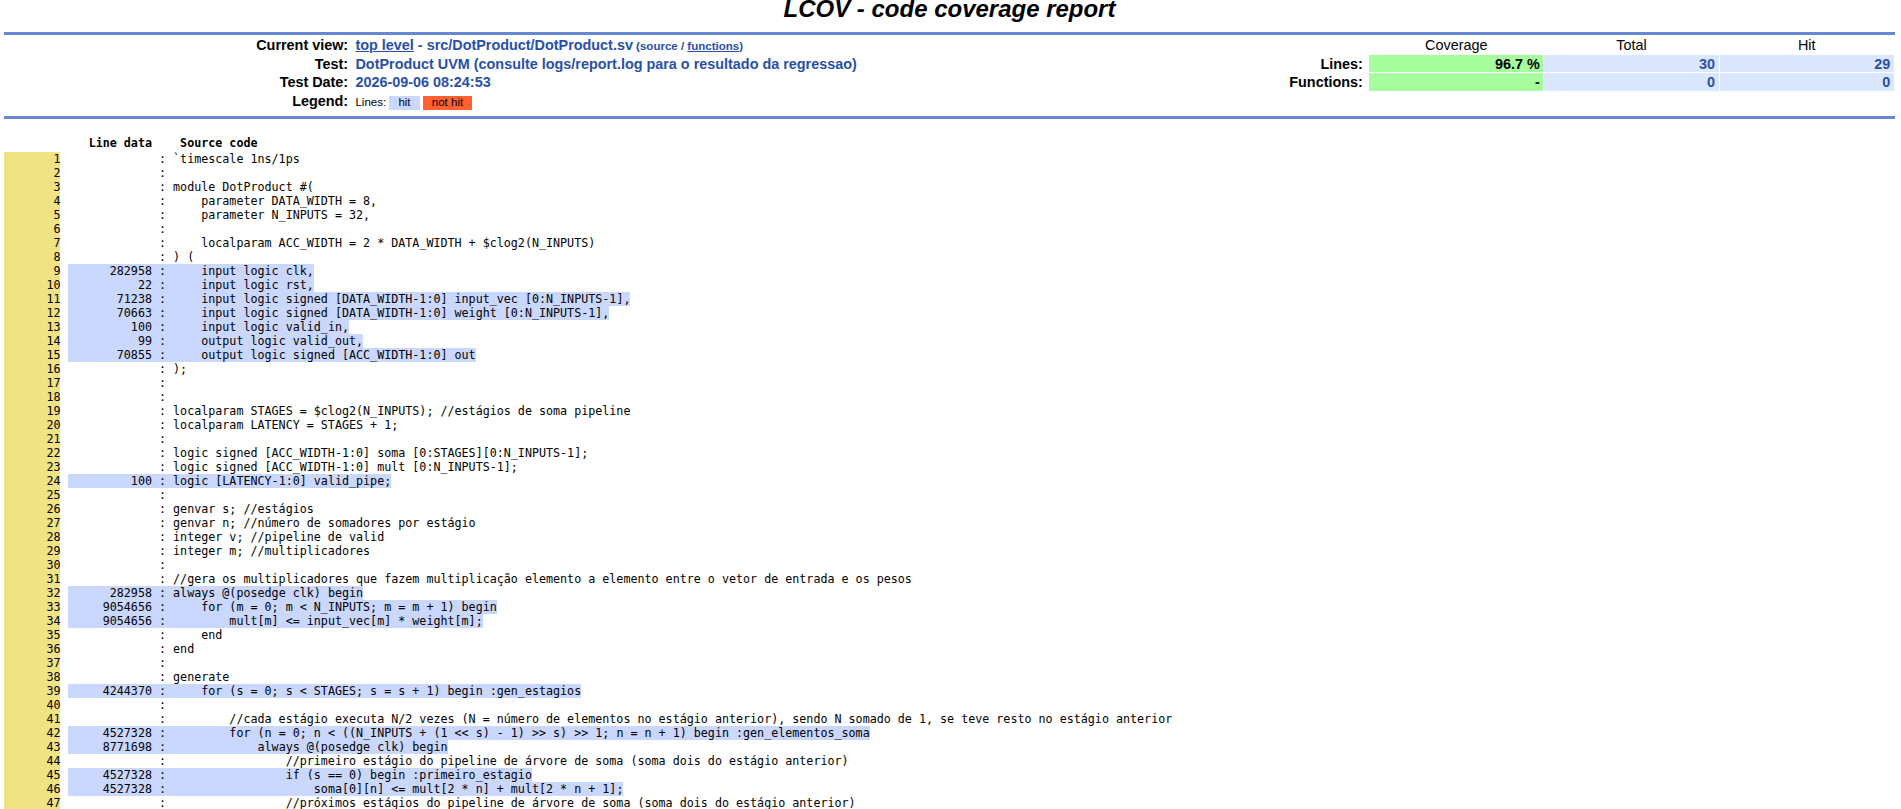
\includegraphics[width=0.94\textwidth,height=0.85\textheight,keepaspectratio]{cap2.png}}
    \caption{Cobertura do DotProduct UVM: detalhamento das linhas do RTL (cap2).}
    \label{fig:dot-cobertura-fonte}
\end{figure}
\clearpage


\subsection{Comentários sobre limitações dos testes}
O espaço completo de entradas e pesos é inviável para verificação exaustiva. As varreduras e amostragens exercitam subespaços representativos, complementados por testes dirigidos. A cobertura de código não substitui os critérios funcionais e temporais.

Após os testes, T07--T11 permaneceram SKIP porque o Verilator utiliza simulação de dois estados e não valida a propagação de X/Z exigida nesses casos. A bancada preserva a política do original: cinco testes obrigatórios não executados produzem \textbf{INCOMPLETE} e retorno de erro. Trata-se de uma limitação do simulador utilizado para esse conjunto de requisitos, e não de comprovação de falha aritmética do bloco.

A precedência de INCOMPLETE no encerramento não apaga a falha de T23 registrada na matriz. É necessário executar X/Z em um simulador UVM de quatro estados e tratar o diagnóstico temporal antes de declarar aprovação completa.


\section{Conclusão}
Apesar da ausência de execução de cinco testes essenciais (T07--T11), considera-se que o bloco está \textbf{aprovado com ressalvas}. Idealmente, deveria ser testada toda a abordagem traçada no plano de verificação; no entanto, devido às limitações da ferramenta utilizada (Verilator) para a simulação de quatro estados, encerra-se aqui esta etapa da verificação.

Essa aprovação com ressalvas não equivale ao atendimento integral dos critérios do plano: permanecem pendentes os testes X/Z e a análise da falha temporal de T23, que não foi demonstrada como defeito do simulador. O resultado automatizado da regressão permanece \texttt{INCOMPLETE}, conforme registrado nas seções anteriores.

\vfill
\begin{center}\textbf{Bloco verificado:} DotProduct -- 32 elementos signed de 8 bits\end{center}
\end{document}
